\documentclass[12pt, letterpaper, twoside]{article}
\usepackage[utf8]{inputenc}
\usepackage[a4paper]{geometry}
\usepackage{array}
\usepackage{booktabs} % For prettier tables
\usepackage{multirow}
\usepackage{multicol}
\usepackage{ragged2e}
\usepackage{xcolor}
\usepackage{gensymb}
\usepackage{fullpage}
\usepackage{hyperref}
\usepackage{amsmath}
\usepackage{scrextend}
\usepackage{graphicx}

\graphicspath{ {./bilder/} }
\newcommand{\cfootnote}[1]{\footnote{\centering #1}}
\title{Bac 2015 Uppgift B1}
\author{Simon Freiermuth \\ \href{mailto:simon@freiermuth.org}{simon@freiermuth.org}}
\date{29 April, 2020}

\begin{document}

%\begin{titlepage}
\maketitle
%\end{titlepage}

\begin{flushleft}
Funktionerna $ f $ och $ g $ definieras av:

\hfill

$ f(x)=0.75x^3 - 1.25x^2 -1 $ och $ g(x) = x^2 - 1 $

\begin{itemize}
%%%%%%%%%%%%%%%%%%%%%%%%%%%%%%%%%%%%%%%%%%%%%%%%%%%%%%%%%%%%%%%%%%%%%%%%%%%%%%%%%%%%%%%%%%%%%%
%   a)
%%%%%%%%%%%%%%%%%%%%%%%%%%%%%%%%%%%%%%%%%%%%%%%%%%%%%%%%%%%%%%%%%%%%%%%%%%%%%%%%%%%%%%%%%%%%%%
	\item[\textbf{a)}]
	Rita graferna till funktionerna $ f $ och $ g $ i samma diagramm. \\
	Beräkna koordinaterna för skärningspunkterna mellan deras grafer.

	\textcolor{red}{
	    $ f(x)=g(x) $
	    $ 0.75x^3 - 1.25x^2 -1 = x^2 - 1 $
	    $ solve(0.75x^3 - 1.25x^2 -1 = x^2 - 1, x) $
	    $ \ \ \ \ \ \rightarrow \{x=0,x=3\} $
	}


	\textcolor{red}{
	    $ g(0) = 0^2-1 = -1 $
	    $ g(3) = 3^2-1 = 8 $
	}


    \textcolor{red}{
        Skärningspunkterna är:
        $ \{0,-1\}, \{3,8\} $
    }

	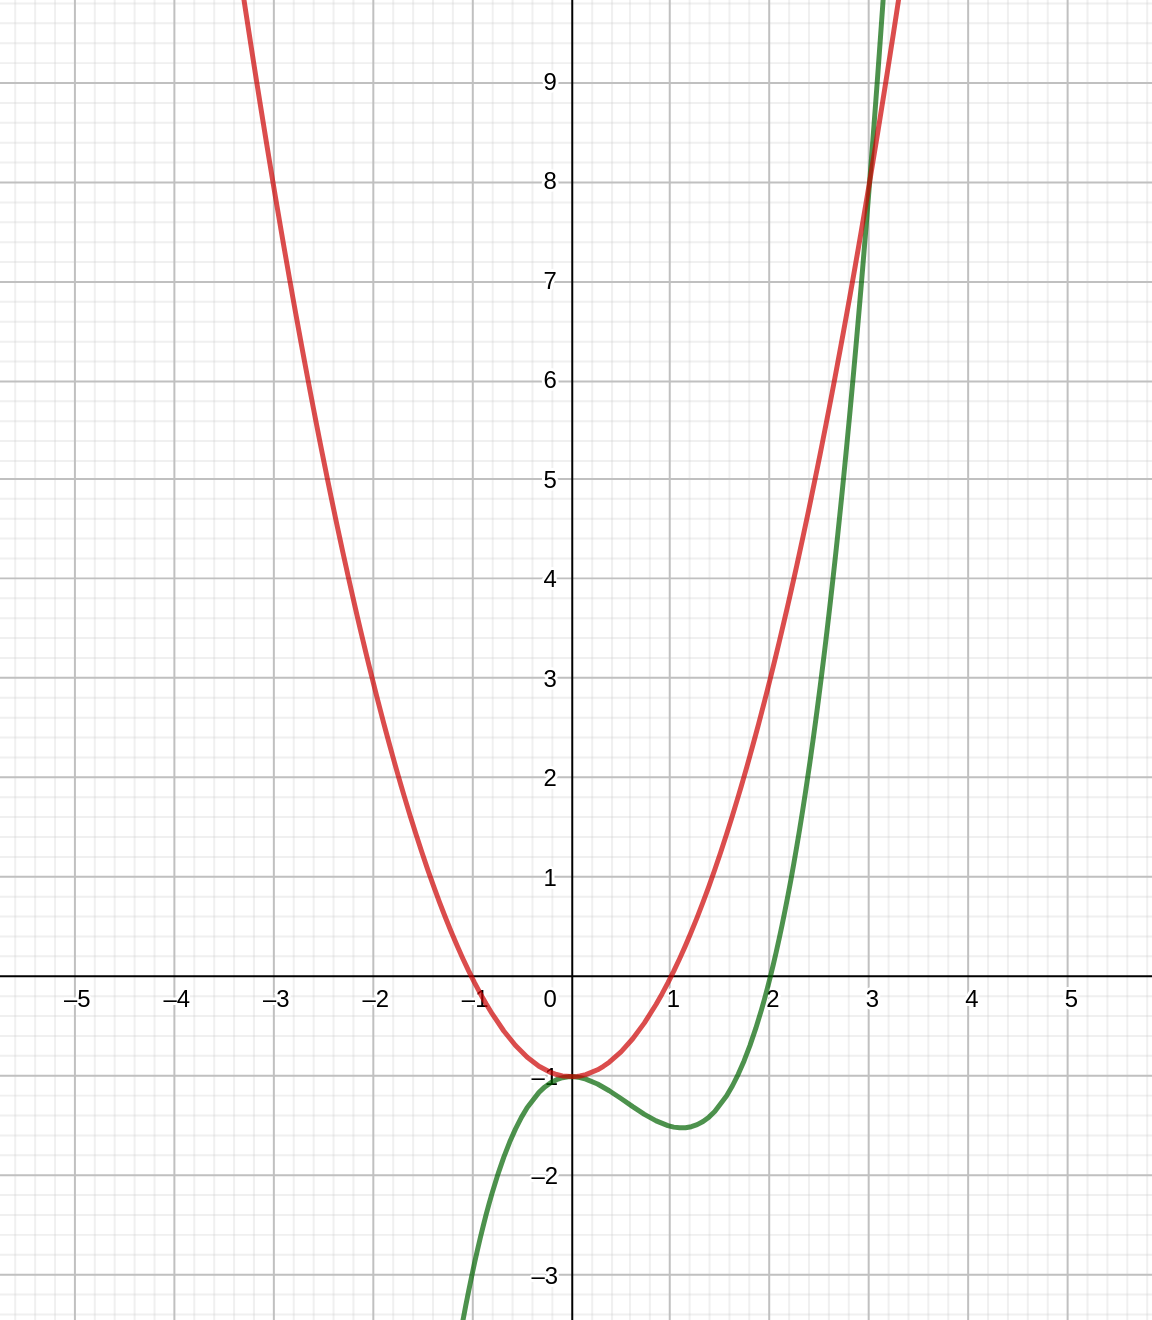
\includegraphics[scale=0.5]{graf1}

	\pagebreak

%%%%%%%%%%%%%%%%%%%%%%%%%%%%%%%%%%%%%%%%%%%%%%%%%%%%%%%%%%%%%%%%%%%%%%%%%%%%%%%%%%%%%%%%%%%%%%
%   b)
%%%%%%%%%%%%%%%%%%%%%%%%%%%%%%%%%%%%%%%%%%%%%%%%%%%%%%%%%%%%%%%%%%%%%%%%%%%%%%%%%%%%%%%%%%%%%%
    \item[\textbf{b)}]
    Beräkna $ \int^3_0(g(x)-f(x))dx $.


    Tolka detta resultat grafiskt.

    \hfill

	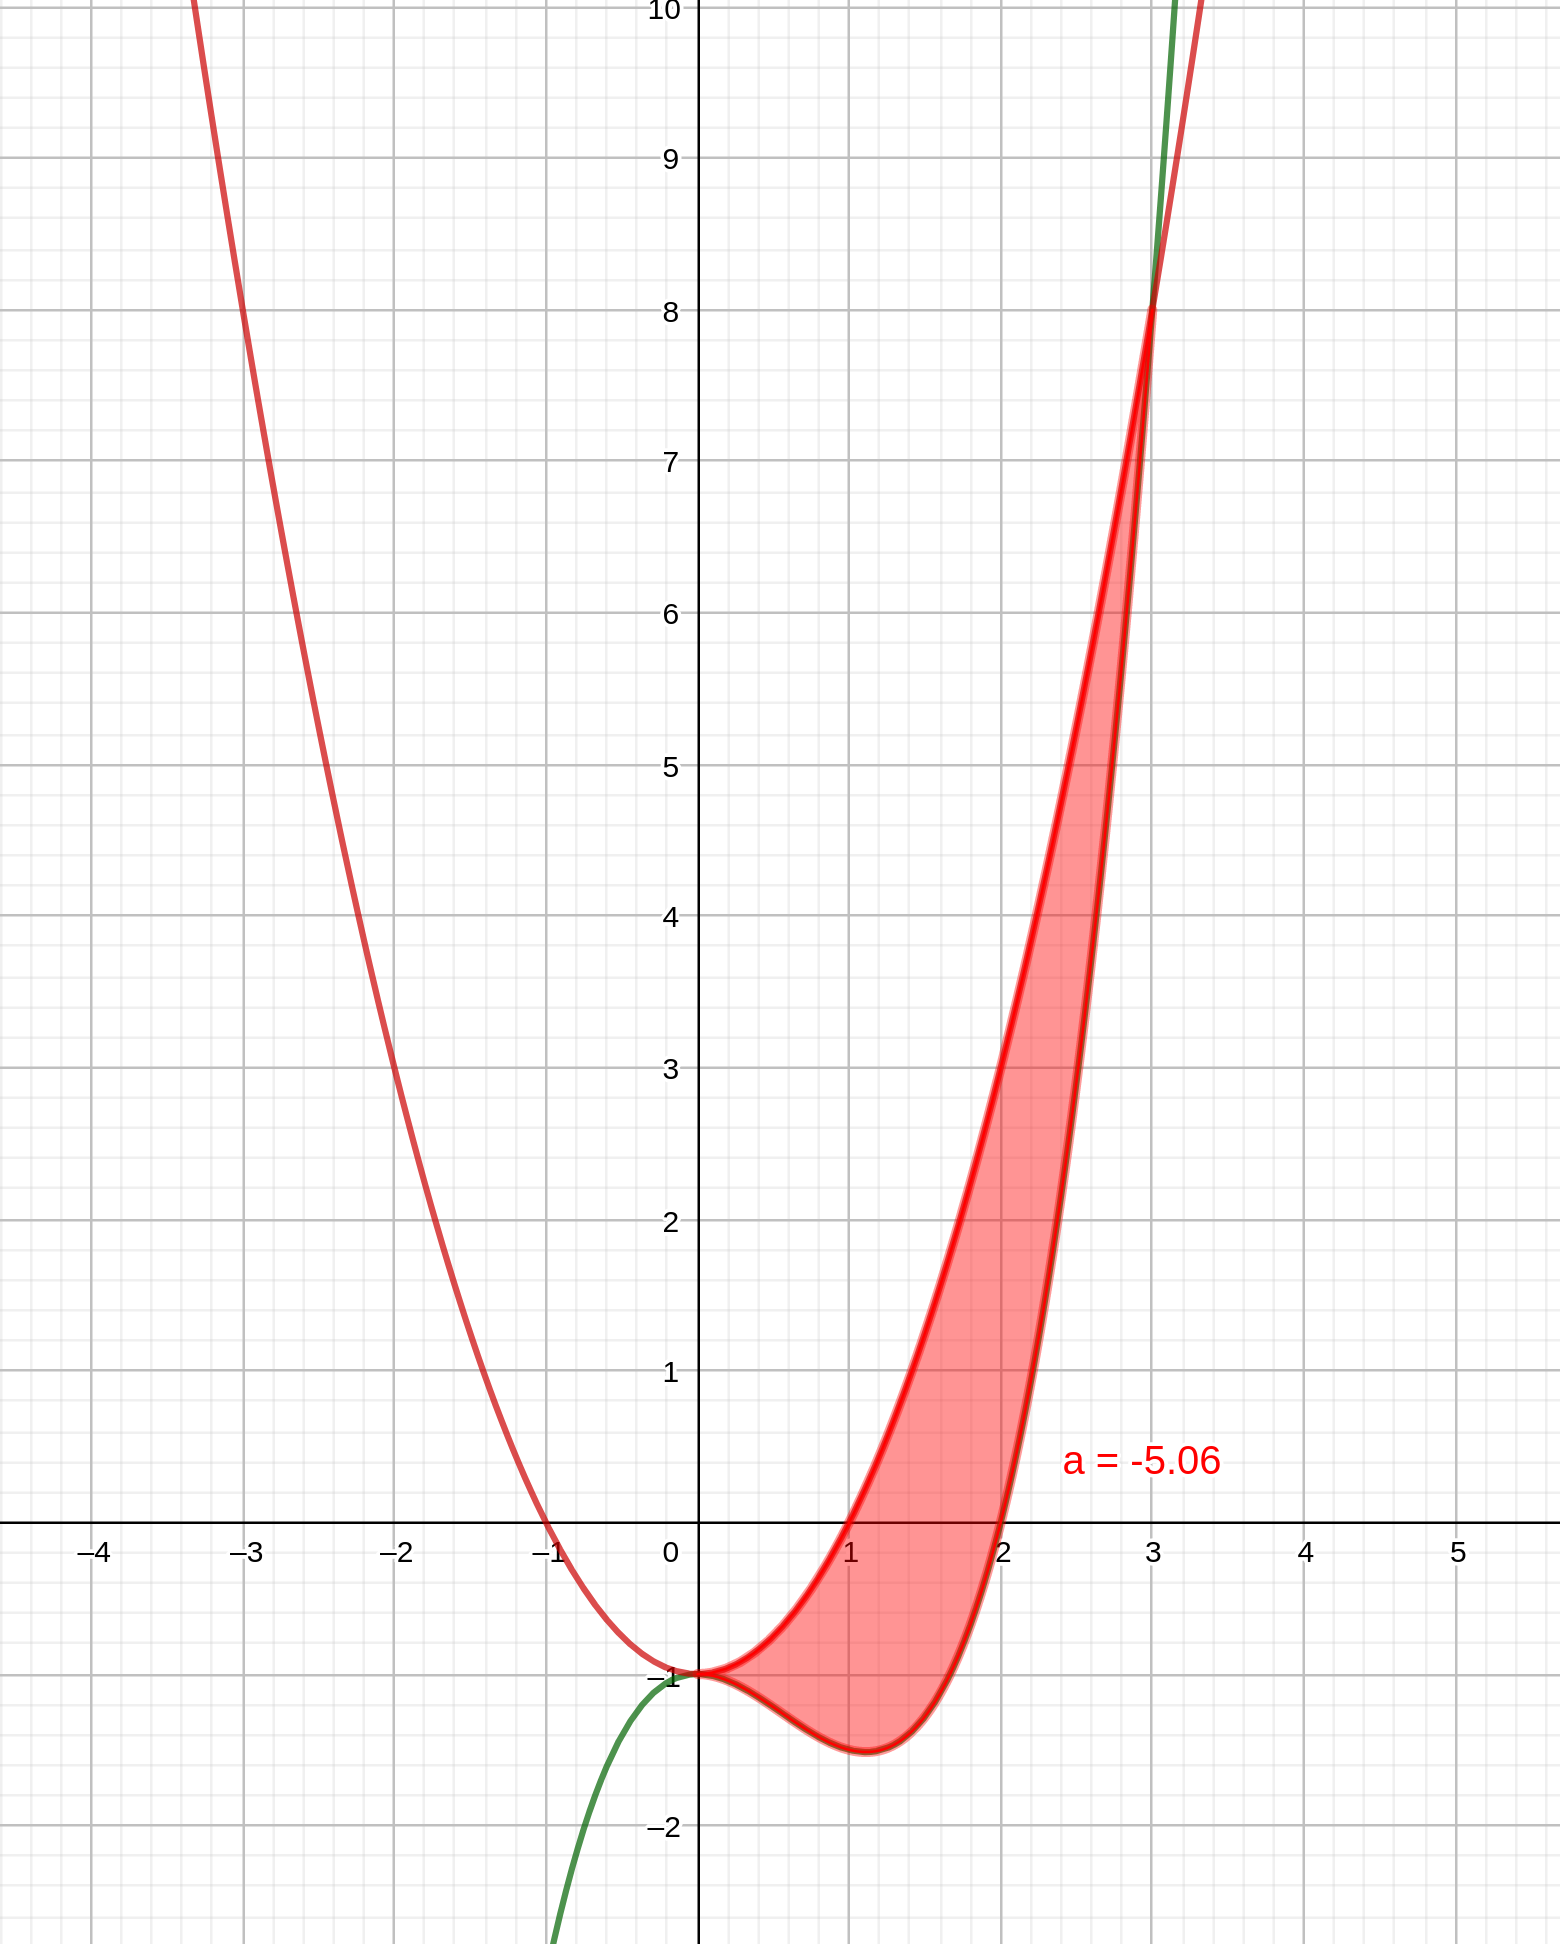
\includegraphics[scale=0.7]{graf2}

	$ area\ =\ 5.06 $

\end{itemize}

\hfill

Båglängden $ L $ av grafen till $ f $ mellan x-värdena $ a $ och $ b $ är givet av formeln:


$$ L = \int_a^b \sqrt{ 1+(f'(x))^2} dx $$

\begin{itemize}

    \item[\textbf{c)}]
    Använd miniräknaren till att bestämma $ L $ när $ a = 0 $ och $ b = 3 $.

    \hfill

    \textcolor{red}{
        $$  L = \int_0^3 \sqrt{ 1+(\frac{d}{dx}(0.75x^3 - 1.25x^2 -1))^2 } dx = 11.12 $$
    }


\end{itemize}

\end{flushleft}
\end{document}
